\documentclass[11pt]{article}

\usepackage{amsmath}
\usepackage{graphicx}
\usepackage{subcaption}

\newcommand{\numpy}{{\tt numpy}}    % tt font for numpy

\topmargin -.5in
\textheight 9in
\oddsidemargin -.25in
\evensidemargin -.25in
\textwidth 7in

\begin{document}

% ========== Edit your name here
\author{Aobo Yang (ay6gv)}
\title{CS6316: HW2}
\maketitle

\medskip

% ========== Begin answering questions here
\begin{enumerate}

\item
Polynomial Regression

1.1 Data Generation

\medskip

The generated data distribution is shown in Figure \ref{fig:data}.

\begin{figure}[!h]
  \centering
  \begin{subfigure}[b]{0.4\linewidth}
    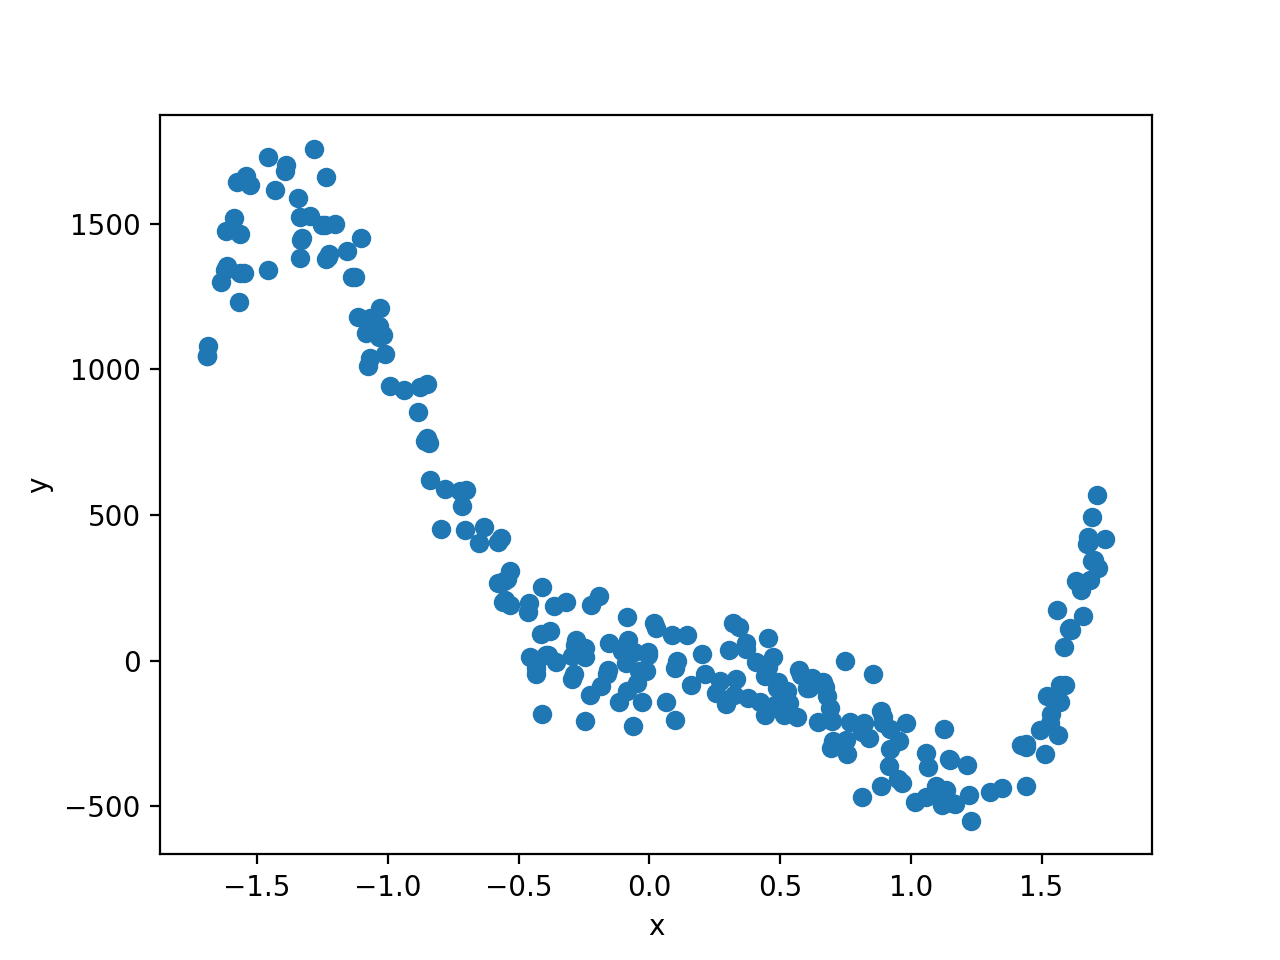
\includegraphics[width=\linewidth]{figures/data_train.png}
    \caption{Training}
  \end{subfigure}
  \begin{subfigure}[b]{0.4\linewidth}
    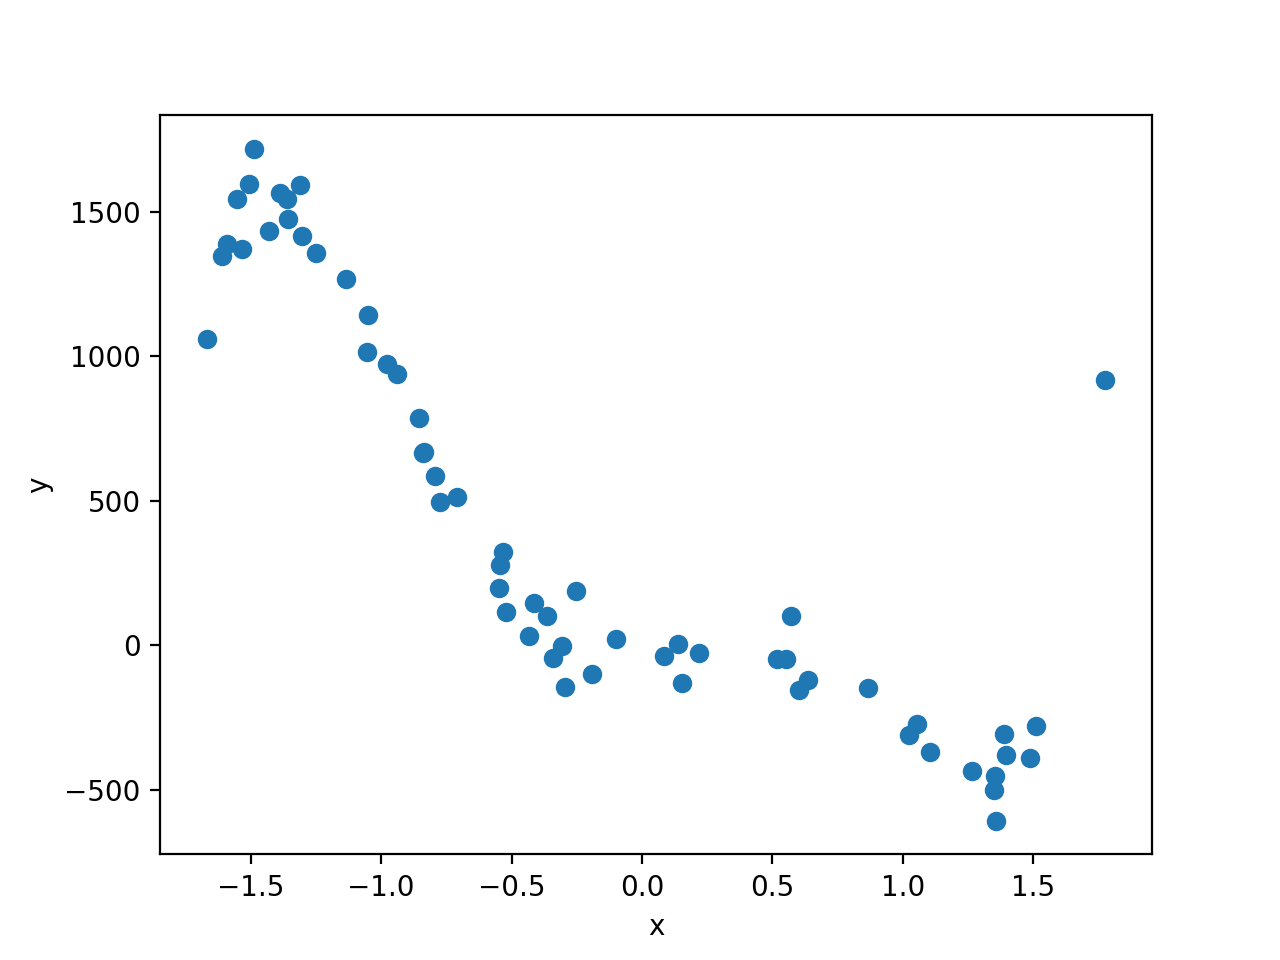
\includegraphics[width=\linewidth]{figures/data_test.png}
    \caption{Testing}
  \end{subfigure}
  \caption{Gradient Descent}
  \label{fig:data}
\end{figure}


1.2 Polynomial Regression Model Fitting

\medskip

The training and validation losses of different polynomial degrees is shown in Figure \ref{fig:poly_order_loss}. The best hyperparamter degree $d$ is $7$.


\begin{figure}[!h]
  \centering
  \begin{subfigure}[b]{0.4\linewidth}
    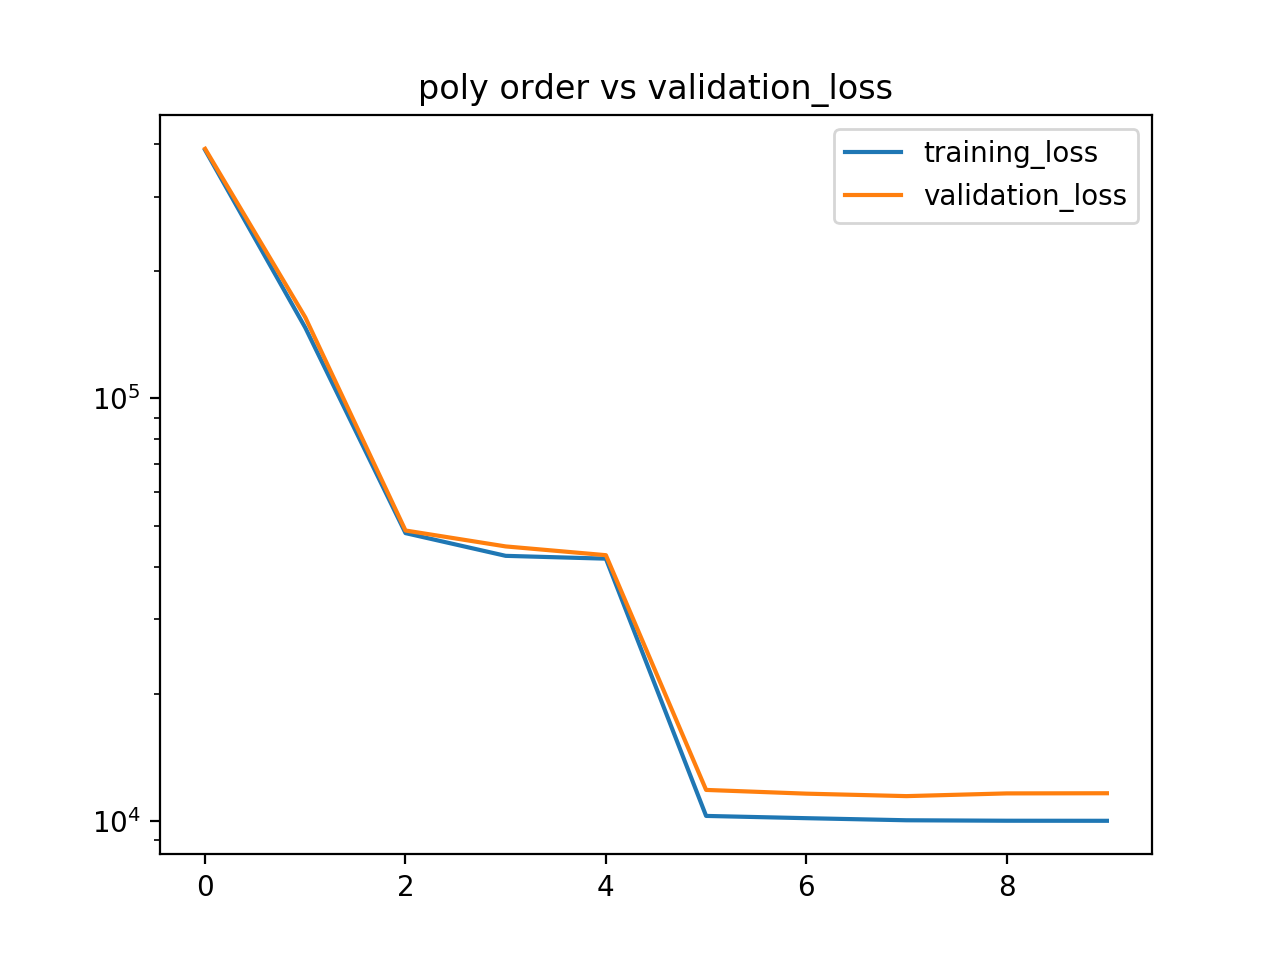
\includegraphics[width=\linewidth]{figures/poly_order_loss.png}
  \end{subfigure}
  \caption{Loss of Polynomial Orders}
  \label{fig:poly_order_loss}
\end{figure}

\medskip

The best $\Theta$ learned is $[-29.60722754,\, -13.93265366,\, 366.49596123,\, -1100.45557026,\, 23.79149025,\,$

$432.79168423,\, -20.91996714,\, -25.45551777]$, which sequentially act as the coefficients of order $0$ to $7$. The testing MSE loss is $8770.13$. The curve is shown in Figure \ref{fig:best_ne}. As required, the best $\Theta$ is gotten in two steps. First, the training data is futher split into training and validation to find the best polynomial order. Second, merge validation back to training and use the whole with normal equation to get this $\Theta$. Comparing with the numbers in data generation, our leaned $\Theta$ is actually reasonable. Although the absolute value scale is quite different, it is because the data has been normalized in data generation. Considering the sign and relative value scale, the learned $\Theta$ matches the data generation. For example, the values for order $6$ and $7$ are negligible, which do not exist in the original data generation.

\begin{figure}[!h]
  \centering
  \begin{subfigure}[b]{0.4\linewidth}
    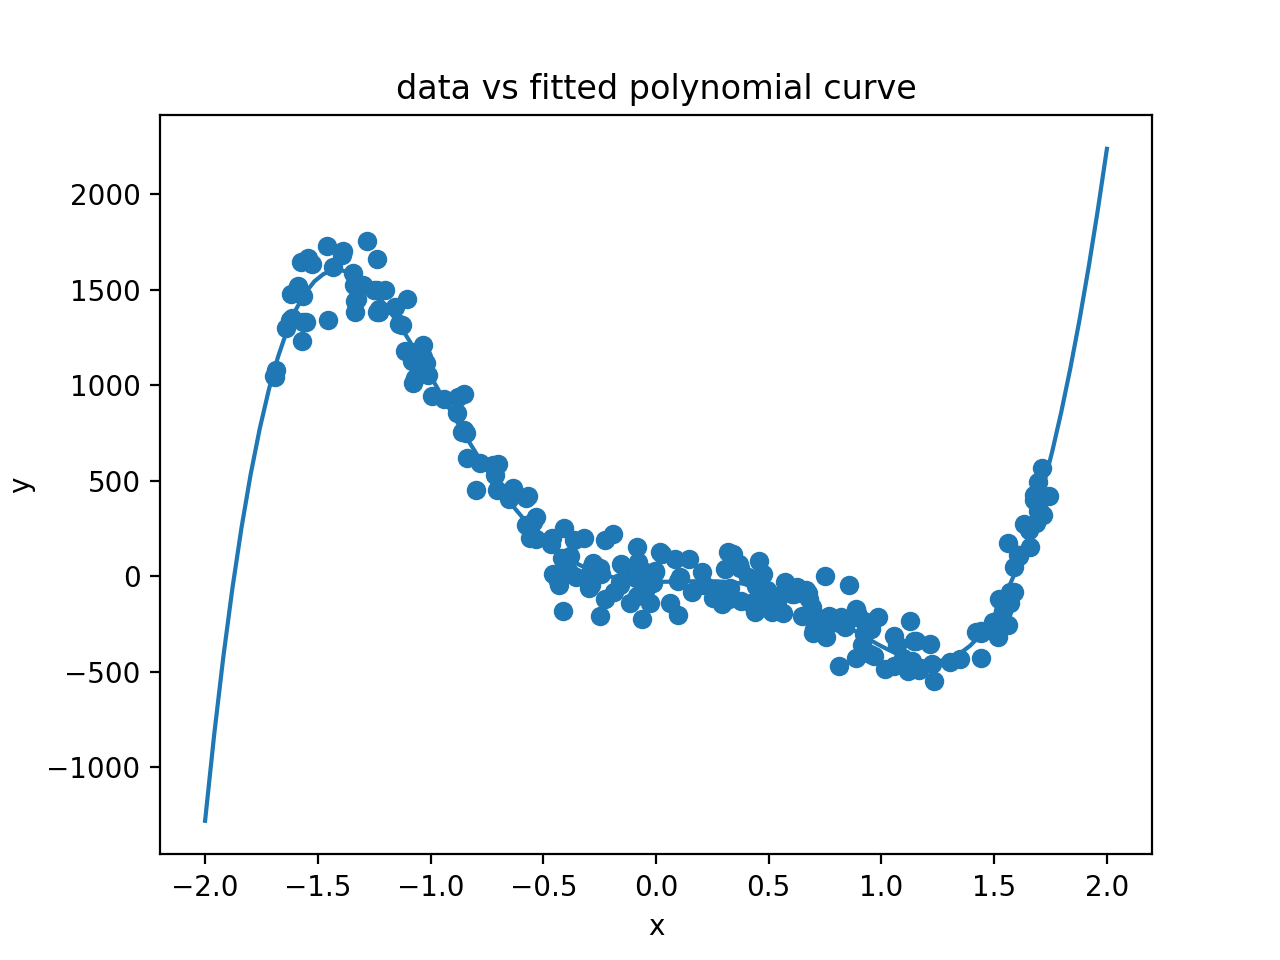
\includegraphics[width=\linewidth]{figures/best_ne_train.png}
    \caption{Training Data}
  \end{subfigure}
  \begin{subfigure}[b]{0.4\linewidth}
    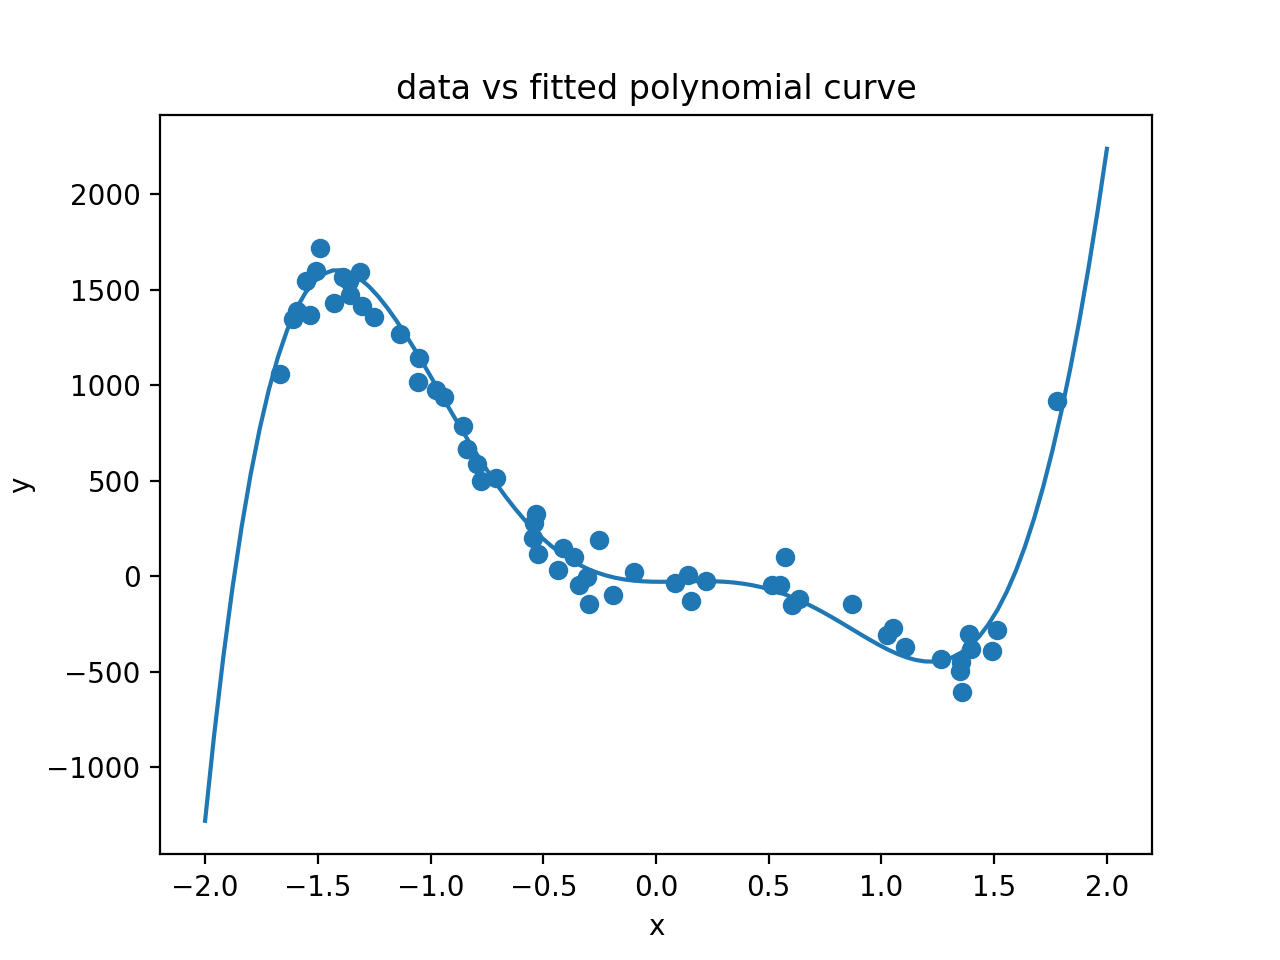
\includegraphics[width=\linewidth]{figures/best_ne_test.png}
    \caption{Testing Data}
  \end{subfigure}
  \caption{Learned Curve}
  \label{fig:best_ne}
\end{figure}

Keeping the degree as $7$, the learned curve and corresponding epoch losses are shown in Firgure \ref{fig:gd_7}. The same plots for degree $2$ is shown in Firgure \ref{fig:gd_2}. The model curve of degree $7$ is much more complex and the end loss is obviously lower then degree $2$. The training loss is lower than validation loss in degree $7$, but in degree $2$, the training loss is even higher. It means the model is too simple and cannot fit the data.

\begin{figure}[!h]
  \centering
  \begin{subfigure}[b]{0.4\linewidth}
    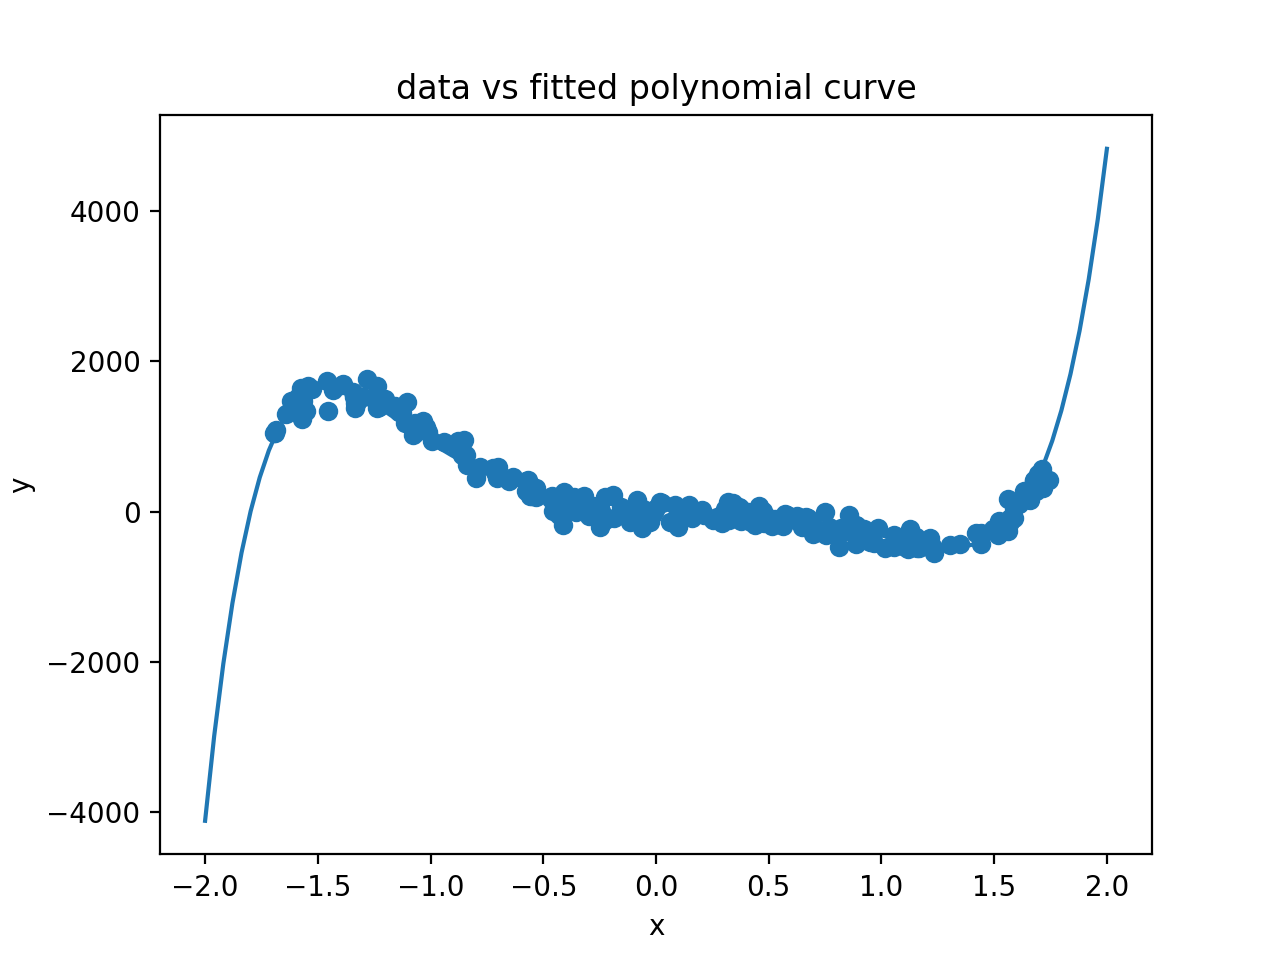
\includegraphics[width=\linewidth]{figures/best_gd_train.png}
    \caption{Training Data}
  \end{subfigure}
  \begin{subfigure}[b]{0.4\linewidth}
    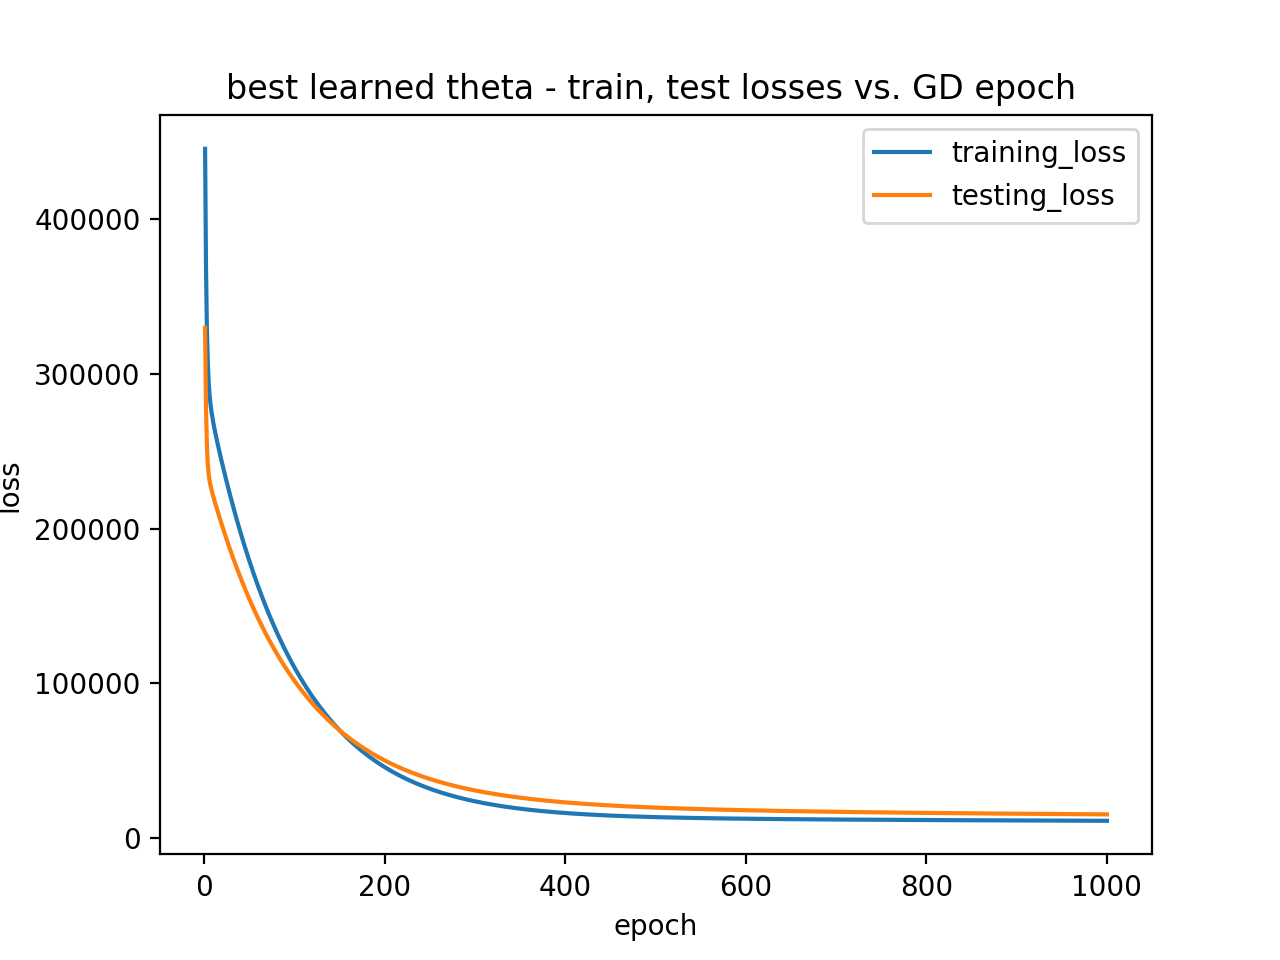
\includegraphics[width=\linewidth]{figures/best_gd_loss.png}
    \caption{Training \& Testing Loss}
  \end{subfigure}
  \caption{Gradient Descent with Degree 7}
  \label{fig:gd_7}
\end{figure}


\begin{figure}[!h]
  \centering
  \begin{subfigure}[b]{0.4\linewidth}
    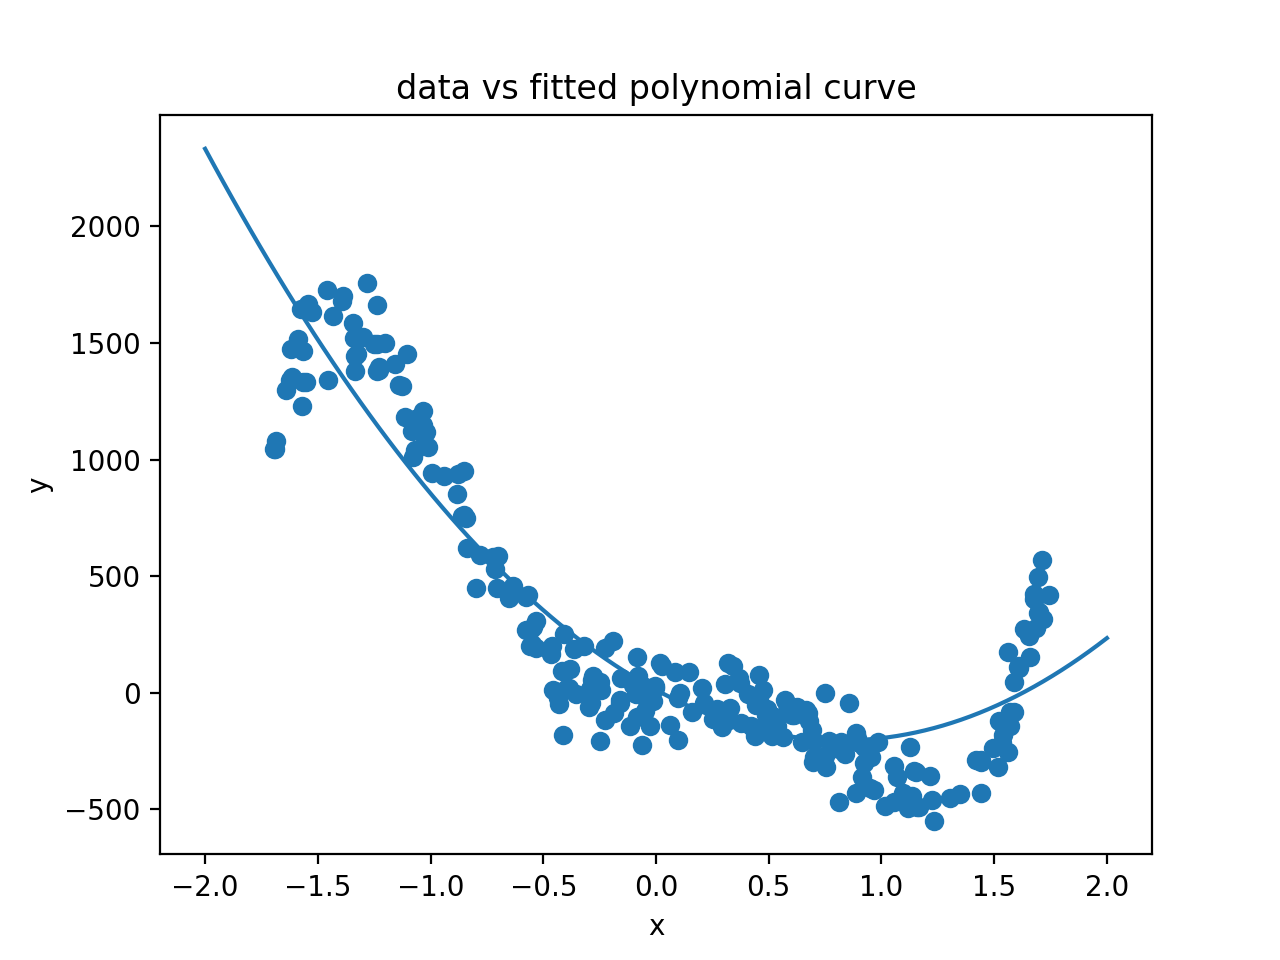
\includegraphics[width=\linewidth]{figures/d2_gd_train.png}
    \caption{Training Data}
  \end{subfigure}
  \begin{subfigure}[b]{0.4\linewidth}
    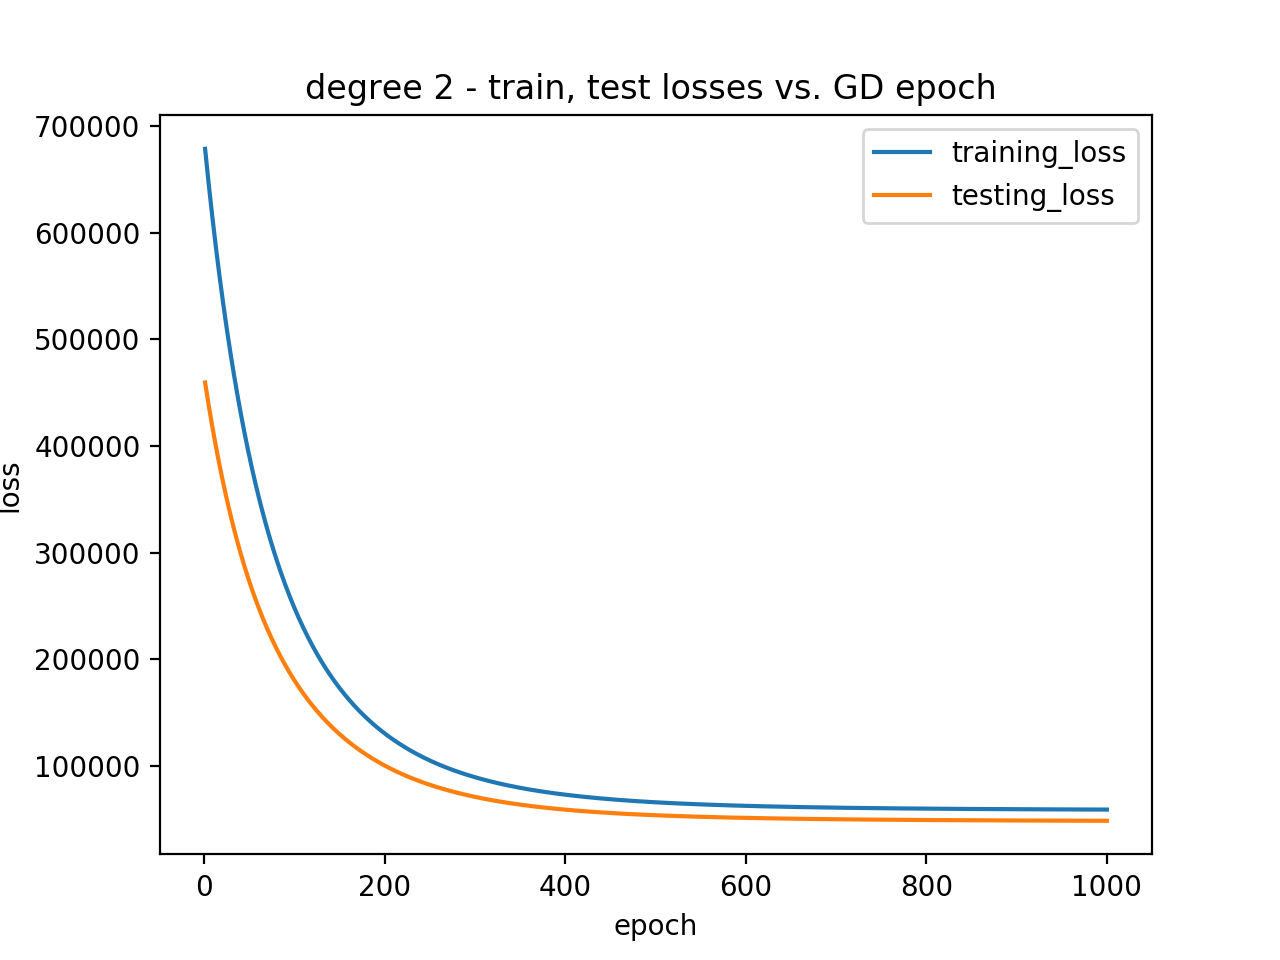
\includegraphics[width=\linewidth]{figures/d2_gd_loss.png}
    \caption{Training \& Testing Loss}
  \end{subfigure}
  \caption{Gradient Descent with Degree 2}
  \label{fig:gd_2}
\end{figure}

The plot of different example size is shown in Figure \ref{fig:example}


\begin{figure}[!h]
  \centering
  \begin{subfigure}[b]{0.4\linewidth}
    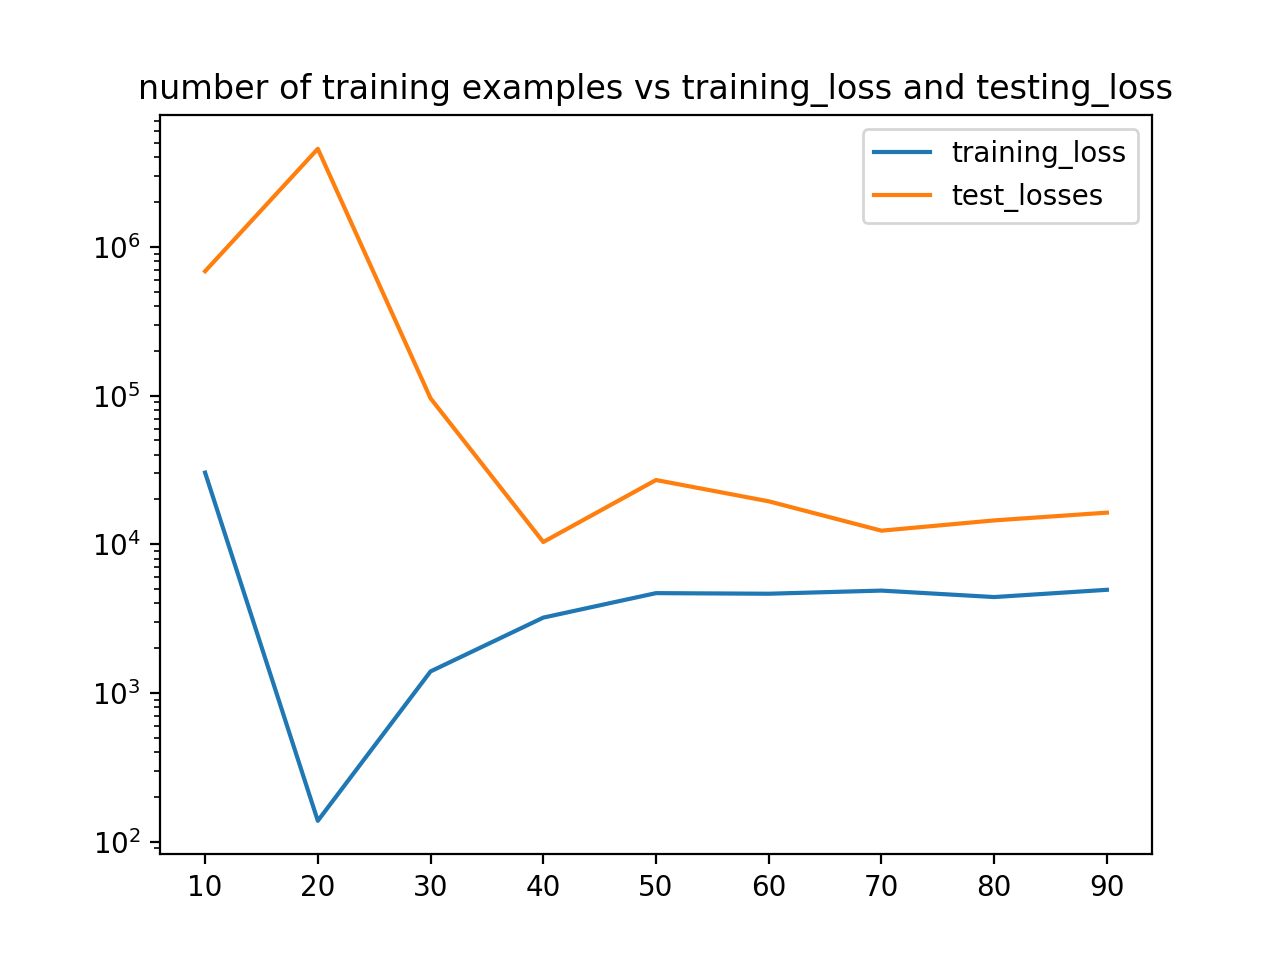
\includegraphics[width=\linewidth]{figures/example_loss.png}
  \end{subfigure}
  \caption{Loss per Example}
  \label{fig:example}
\end{figure}

\item
Ridge Regression

2.2


\medskip
3.3



% ========== Continue adding items as needed

\end{enumerate}

\end{document}
\grid
\grid
